% !TeX spellcheck = pl_PL
\newpage
\section{System przechowywania \newline danych}
Rozdział ten przedstawia propozycję systemu przechowywania danych. Struktura sieci informatycznej jest rozbudowana, zatem aby scentralizować dostęp do danych zastosowano technologię NAS.

\subsection{Struktura NAS}
Dostęp do serwera NAS nie wymagają telefony IP oraz bramka VoIP, zatem nie zostały uwzględnione w strukturze. Schemat systemu NAS znajduje się na rysunku \ref{schemat:schemat_sieci_NAS}. Połączenia pomiędzy stacjami roboczymi poprowadzone są poprzez iSCSI (wykorzystując sieć przewodową).
\begin{landscape}
	\hspace{4cm}
	\begin{figure}[!h]
		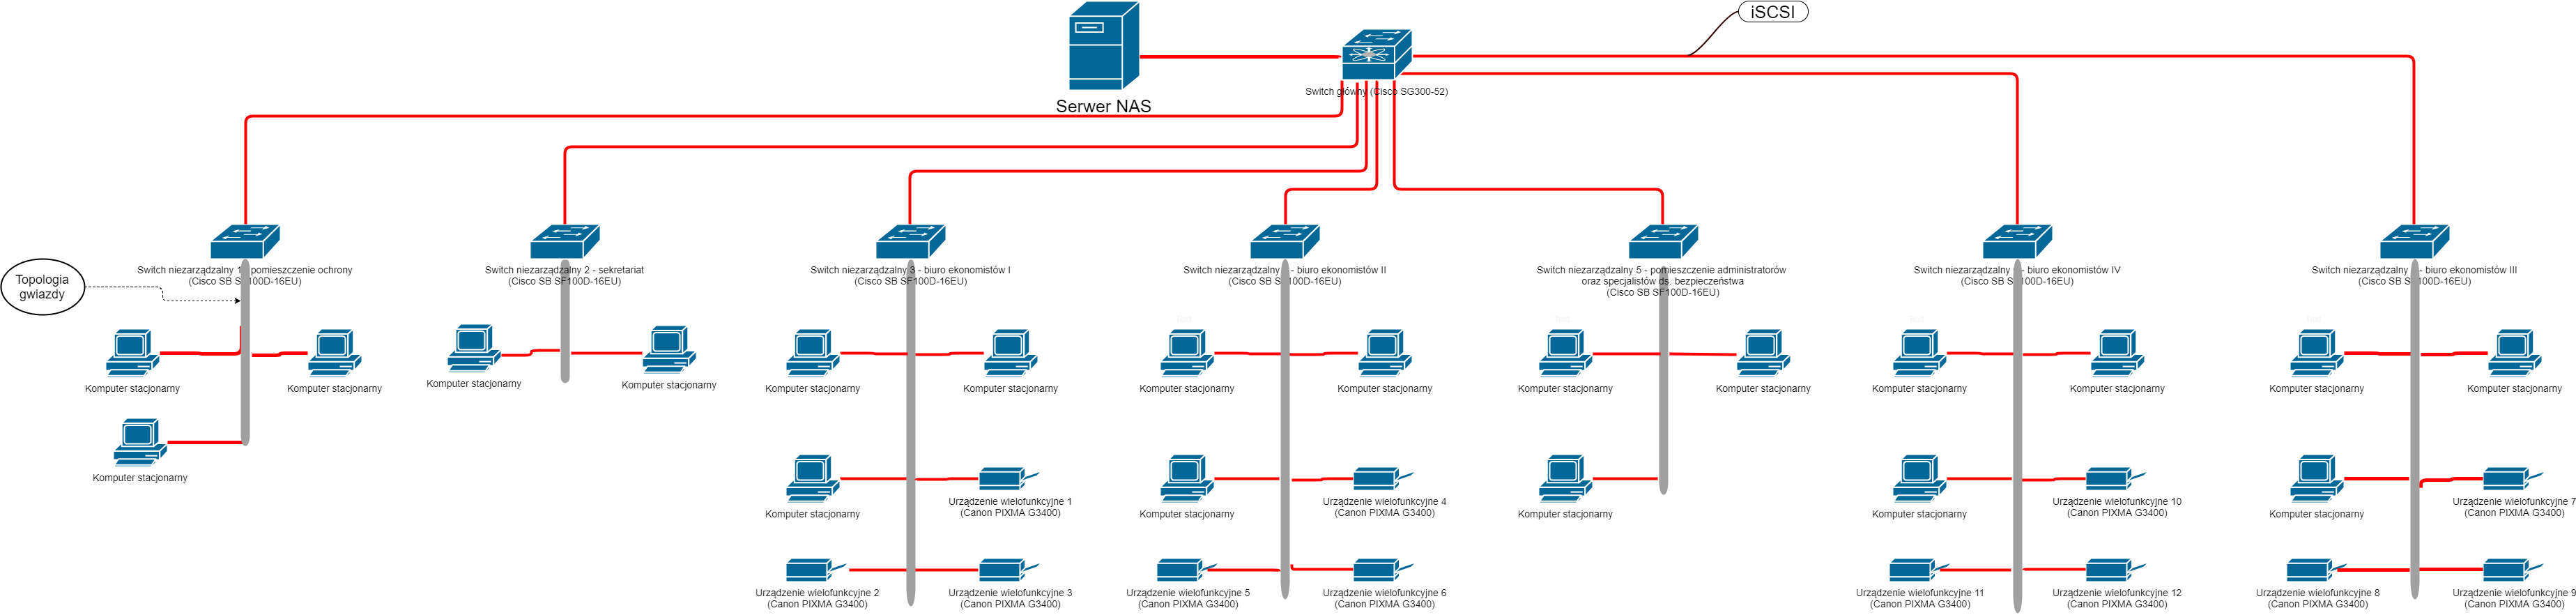
\includegraphics[width=24cm]{Schemat_NAS.png}
		\caption{Schemat struktury NAS}
		\label{schemat:schemat_sieci_NAS}
	\end{figure}
\end{landscape}

\subsection{Serwer}
Serwer główny ze względu na potrzebę niezawodności pracy posiada macierz dyskową RAID 4 z 3 dyskami HDD WD Red 2TB. W przypadku awarii dowolnego dysku istnieje możliwość odtworzenia utraconych danych. Jest to wolniejsze rozwiązanie niż powiedzmy RAID 5, ale zapewnia większe bezpieczeństwo w przypadku uszkodzenia. Wykorzystując daną macierz dyskową posiadamy 4TB pojemności dyskowej, wg podanych informacji od zleceniodawców taki rozmiar pamięci powinien wystarczyć na przechowywanie danych przez 50 lat (jest to okres przez jaki należy przechowywać dane księgowe).

Serwer zapasowy posiada kompletną kopię macierzy dyskowej z serwera głównego zapewniając redundancję w przypadku całkowitej awarii sprzętu. W~ten sposób zabezpieczamy w znacznym stopniu dane przed utraceniem.

Na serwerze w środowisku wirtualnym uruchomiony jest system FreeNAS odpowiedzialny za zarządzanie przechowywaniem plików. W systemie FreeNAS uruchomione są usługi odpowiedzialne za replikację danych oraz tworzenie kopii zapasowych. Pełna kopia zapasowa będzie wykonywana w każdy poniedziałek, natomiast kopia przyrostowa będzie wykonywana w pozostałe dni tygodnia. Każda kopia zapasowa będzie szyfrowana algorytmem AES.

Dodatkowo kopie zapasowe z okresu powyżej roku przechowywane są na taśmach magnetycznych w pomieszczeniu archiwum.

\subsection{Komputery pracowników}
Komputery pracowników ze względu na nie zbyt wysoką szkodliwość utraty danych (pod warunkiem przenoszenia danych systematycznie do pamięci serwera - NAS) nie wymagają szczególnych zabezpieczeń. Wykorzystano dwa rodzaje dysków: HDD WD Black 500GB dla plików oraz SSD Samsung 850 Pro 120GB dla wybranych programów oraz systemu operacyjnego. W przypadku braku dwóch slotów dyskowych drugi dysk (HDD) zastępuje napęd optyczny. Magistralą użytą w komputerach jest SATAIII ze względu na parametry techniczne komputerów (brak magistrali NVIe).


\section{Trwałe usuwanie danych}
Na nośnikach danych w postaci dysków twardych i taśm magnetycznych przechowywane są wrażliwe dane osobowe oraz dane dotyczące przedsiębiorstwa. Aby, takie dane nie trafiły w niepowołane ręce podczas wymiany sprzętu czy też jego awarii, należy zadbać o bardzo ważny aspekt jakim jest trwałe usunięcie danych z nośników. Wyróżnia się dwie metody usuwania danych: programową oraz sprzętową. W przypadku, gdy nośnik jest sprawny, zaleca się użycie odpowiedniego programu (Acronis Drive Cleanser), który w sposób bezpieczny trwale usunie dane. Taka metoda usuwania danych jest nie tylko tańsza, ale też skuteczniejsza i bezpieczniejsza dla środowiska niż metoda fizyczna. Metodę sprzętową zaleca się używać, gdy nośnik danych jest niesprawny. Jedną z najbardziej skutecznych metod fizycznych usuwania danych jest wykorzystanie wysokiej temperatury powyżej 1000 stopni Celsjusza. Przy poprawnym procesie usuwania za pomocą odpowiedniej temperatury, nie da się odczytać danych w warunkach domowych i laboratoryjnych.
